%!TEX program = xelatex
%!TEX TS-program = xelatex
%!TEX encoding = UTF-8 Unicode

\documentclass[a4paper]{article}
\usepackage[UTF8, heading = false, scheme = plain]{ctex}
\usepackage{graphicx}
\usepackage{cite}
\usepackage{geometry}
\geometry{left=2.0cm, right=2.0cm, top=2.5cm, bottom=2.5cm}
\usepackage[colorlinks,linkcolor=red,anchorcolor=blue,citecolor=green]{hyperref}
\usepackage{subfig}
\usepackage{caption}
\captionsetup{font={scriptsize}}

\renewcommand\figurename{图}

\makeatletter
\let\@afterindentfalse\@afterindenttrue
\@afterindenttrue
\makeatother
\setlength{\parindent}{2em}  

\linespread{1.4}
\setlength{\parskip}{0.5\baselineskip}
\usepackage{bm}

\title{学习汇报\\第六周}
\author{熊凯亚}
\date{\today}

\begin{document}
\maketitle
\paragraph{回顾}
上周主要看了关于联合学习的隐私保护的文章。对于联合学习的隐私问题,\cite{bonawitz2017practical}提出了一种能够保护用户隐私的安全聚集算法。不同于协作学习,联合学习中的参与者是一些移动设备,这些移动设备有一些特殊的属性,比如随意性,移动设备会随时失去网络连接,随时退出模型的训练等等。

联合学习原理安全聚集算法原理如下:中心化学习中,用户设备和云端模型交互,使用设备数据提高模型的准确性。联合学习中,用户设备下载云端模型,并在本地使用设备数据训练模型,并上传至云端更新模型。联合学习中,假设云服务提供商(Google)为恶意敌手。使用了安全聚集算法之后,模型更新的聚集由虚拟的第三方通过安全多方计算来完成,这就保证了云服务提供商对聚集的模型更新的不可知性。
\begin{figure*}[!h]
\begin{tabular}{ccc}
\subfloat[传统中心化云端训练模型]{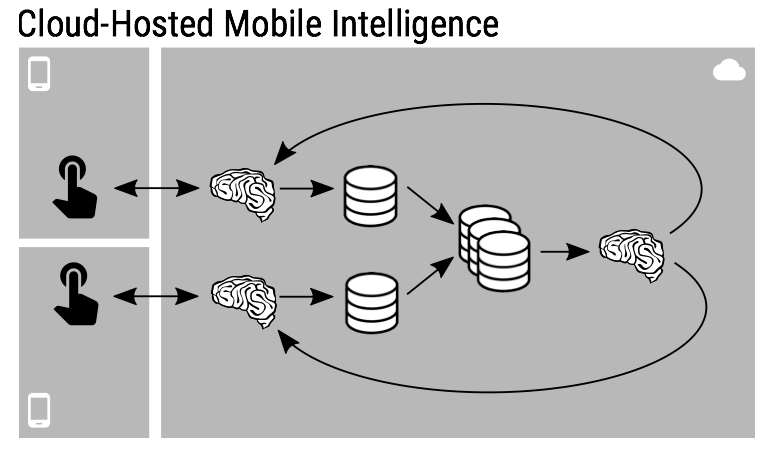
\includegraphics[width = 2in]{fig/Cloud-Hosted_Mobile_Intelligence.png}}&
\subfloat[联合学习]{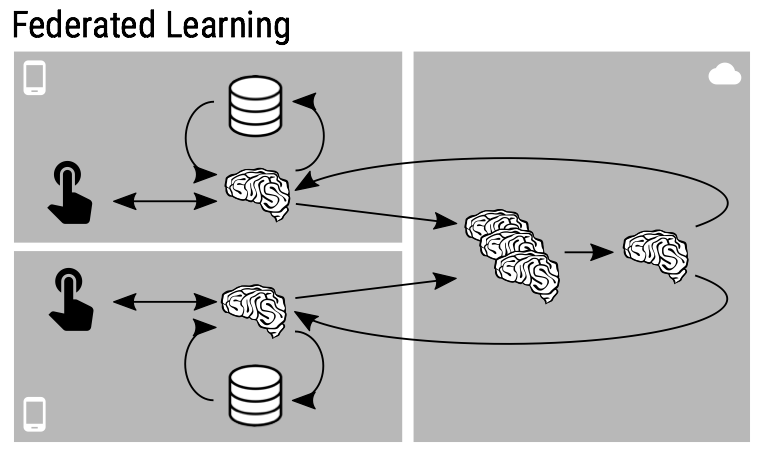
\includegraphics[width = 2in]{fig/Federated_Learning.png}}&
\subfloat[使用安全聚集的联合学习]{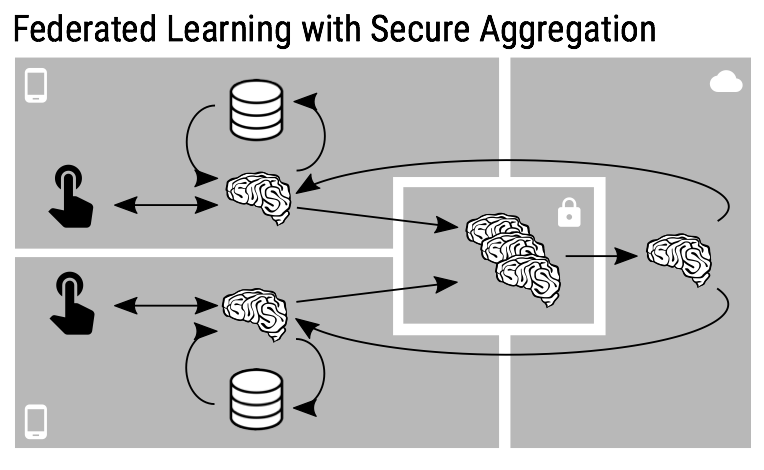
\includegraphics[width = 2in]{fig/Federated_Learning_with_Secure_Aggregation.png}}
\end{tabular}
\end{figure*}

安全聚集算法中,对于用户设备使用本地数据在本地训练的模型更新,使用秘密分享协议(Secret Sharing)将模型更新分为n份上传至云端服务器,并在服务器端使用安全多方计算,计算多个设备上传的模型更新。然后将计算结果添加到已有模型上,随后各个设备再继续下载最新的模型在本地训练,如此循环,直至模型收敛。


\paragraph{协作深度学习网络}
联合学习与协作学习类似,因此本周主要看了最初提出协作深度学习的文章\cite{shokri2015privacy},了解了一下关于协作深度学习的工作原理。
典型的多层网络中:\\
1.每个神经元会接收到上层神经元的输出加上来自一个特殊神经元的偏移信号,然后根据它的输入计算加权平均值,称为总输入。通过总输入值应用非线性激活函数来计算神经元的输出。\\
2.K层的神经网络输出向量为$\bm{a}_k=f(W_k\bm{a}_{k-1})$,其中$f$为激活函数,$W_k$为权重矩阵,它决定了每个输入信号的权重。
常用的激活函数有如下几个:
\begin{itemize}
\item 双曲正切 $f(z)=(e^{2z}-1)(e^{2z}+1)^{-1}$
\item Sigmoid $f(z)=(1+e^{-z})^{-1}$
\item Rectifier $f(z)=max(0,z)$
\item Softplus $f(z)=log(1+e^z)$
\end{itemize}
3.最后一层的激活函数通常是Softmax函数$f(z_j)=e^{z_j}(\Sigma_ke^{z_k})^{-1},\forall j$ \\
4.最后一层中,每个神经元$j$的输出就是输入属于类$j$的概率。\\
5.越高层计算出的值表示数据的特征越抽象。\\
6.若神经网络用于分类,抽象特征也代表输入输出的关系。\\
7.深度学习的主要挑战是从训练数据中自动学习使神经网络的目标(例如分类的准确性)最大化的参数值(权重矩阵)。\\
8.梯度下降始于随机点(由神经网络的参数决定),然后每步计算被优化的非线性函数的梯度并更新参数以减少梯度。一直持续到算法收敛到局部最优。\\
9.每个权重参数的梯度由feed-forward前向反馈和back-prapagation后向传播过程计算出来。
\paragraph{DSSGD}
本文使用了一种叫做分布式选择随机梯度下降的算法(Distributed Selective Stochastic Gradient Descent),此算法用来在参与者分享参数时,决定选择性分享部分参数梯度。\\
算法执行步骤如下图:\\
\begin{figure*}[!h]
\begin{tabular}{cc}
\subfloat[参与者执行步骤]{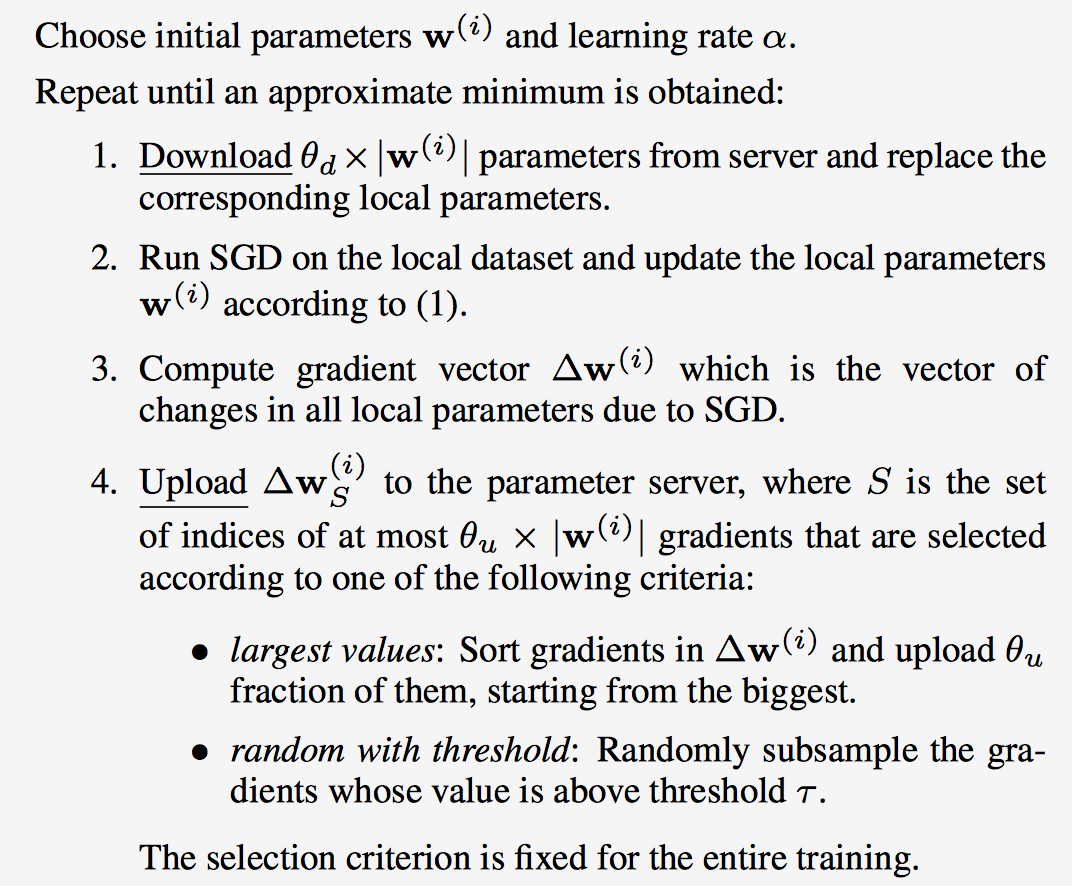
\includegraphics[width = 3.4in]{fig/DSSGD_participant.png}}&
\subfloat[参数服务器执行步骤]{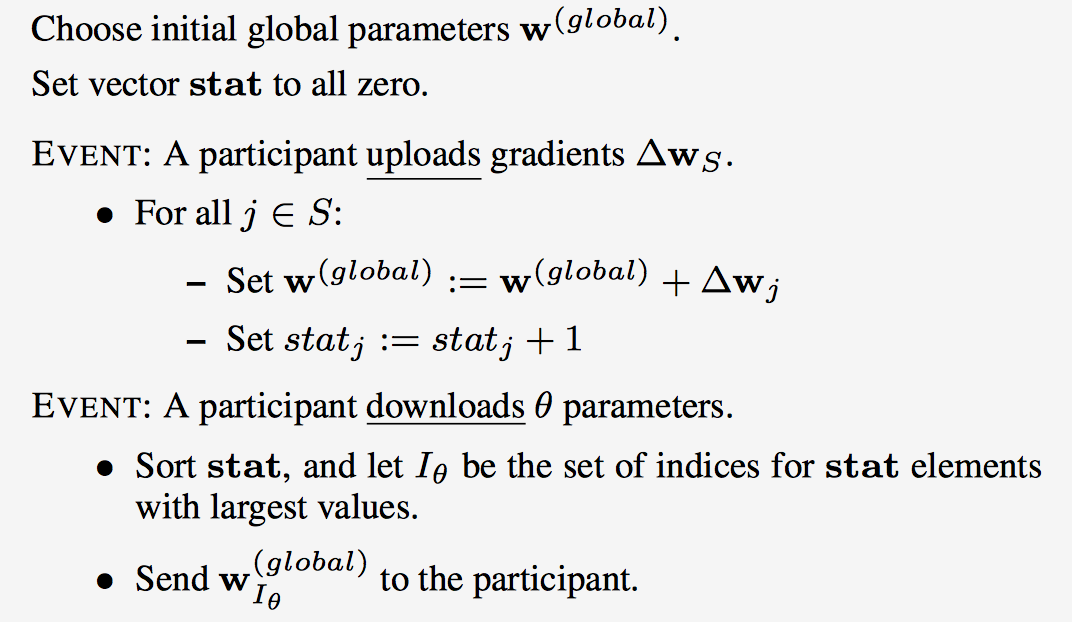
\includegraphics[width = 3.4in]{fig/DSSGD_server.png}}
\end{tabular}
\caption{DSSGD算法执行步骤}
\end{figure*}

\paragraph{参与者执行步骤}
选择初始参数$\bm{w}^{(i)}$和学习速率$\alpha$.
重复下列步骤,直至最小值出现:
\begin{enumerate}
\item 从服务器下载参数$\theta_d\times|\bm{w}^{(i)}|$并替换相应的本地参数.
\item 在本地数据集上运行SGD并根据步骤一更新本地参数$\bm{w}^{(i)}$.
\item 计算梯度向量$\triangle\bm{w}^{(i)}$
\item 上传$\triangle\bm{w}_S^{(i)}$到服务器,其中$S$是根据下列规则选出来的最多$\theta_u\times|\bm{w}^{(i)}|$
梯度的索引的集合。
	\begin{itemize}
	\item 最大值:将$\triangle\bm{w}^{(i)}$中的梯度排序并从最大的开始上传$\theta_u$部分梯度。
	\item 阈值随机:随机选择低于阈值$\tau$的梯度。
	\end{itemize}
\end{enumerate}

\paragraph{参数服务器执行步骤}
选择初始全局参数$\bm{w}^{(global)}$,设置向量$\bm{stat}$至全零。
对于参数服务器来说,有两个事件,一个是参与者上传了梯度$\triangle\bm{w}_S$,另一个是参与者下载了参数$\theta$。\\
参与者上传梯度$\triangle\bm{w}_S$:
\begin{itemize}
\item 对于所有$j\in S$:
	\begin{enumerate}
	\item 令$\bm{w}^{(global)}:=\bm{w}^{(global)}+\triangle\bm{w}_j$
	\item 令$stat_j:=stat_j+1$
	\end{enumerate}
\end{itemize}
参与者下载参数$\theta$:
\begin{itemize}
\item 对$stat$排序,并令$I_\theta$为有最大值的$stat$元素索引的集合.
\item 将$\bm{w}_{I_\theta}^{(global)}$发送给参与者.
\end{itemize}

% \paragraph{加入差分隐私}
% 本文采用了选择性分享参数来避免模型训练参与者的隐私遭到泄露。但是实现表明还是有一小部分数据会被间接地泄露出去,因此可以在分享参数时在其中加入噪声。步骤如下:
% \begin{figure*}[!ht]
% 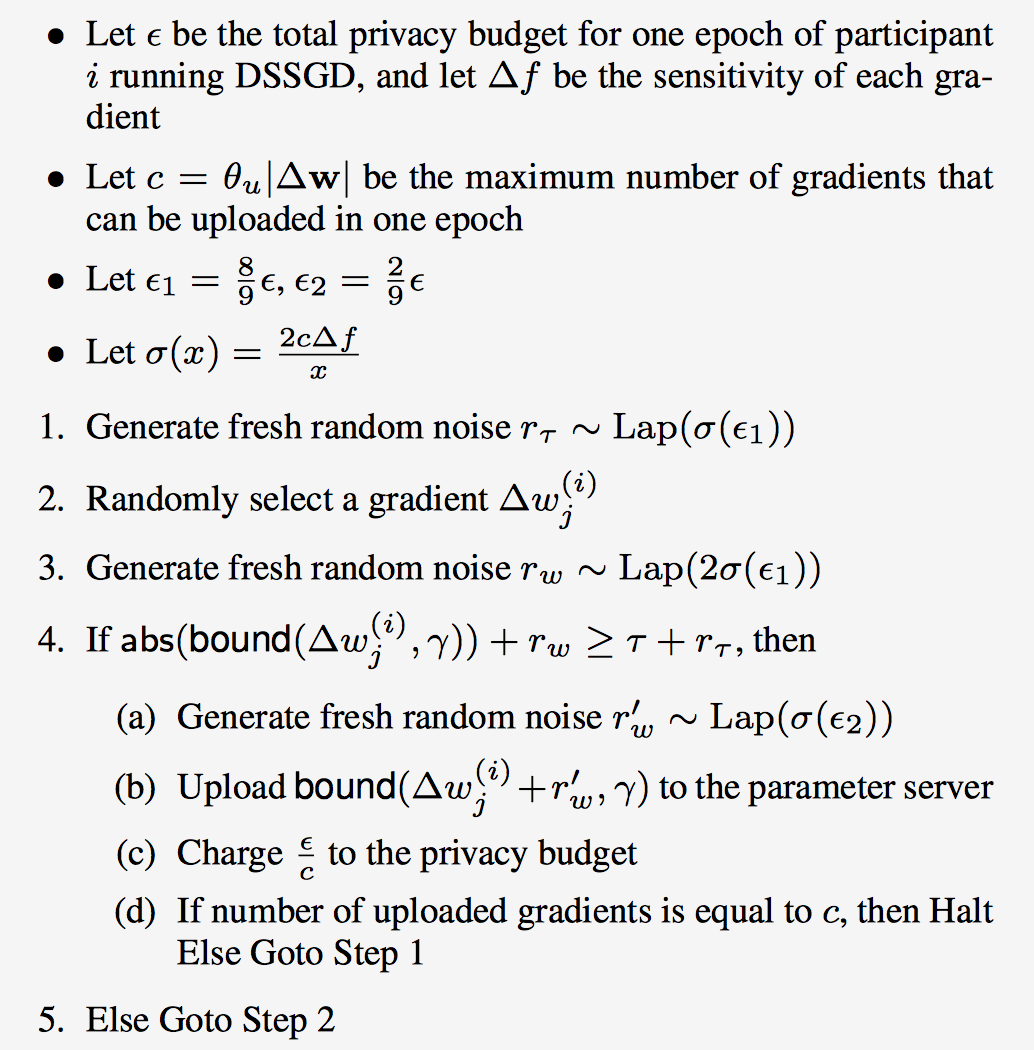
\includegraphics[width = 3.4in]{fig/DSSGD_DP.png}
% \caption{加入差分隐私的DSSGD}
% \end{figure*}
\bibliographystyle{IEEEtran}
\bibliography{references}
\end{document}
